\documentclass{bmd2016p}

\begin{document}

\begin{center}
\fontsize{14}{20}{\bf Instructions for Preparing a Paper for \\[3pt]
                      the Bicycle and Motorcycle Dynamics Symposium Proceedings}
\end{center}

%%%%%%%%%%%%%%%% authors %%%%%%%%%%%%%%%
\begin{center}
\normalsize{\bf{A. B. Authorone$^{*}$, C. Authortwo$^\#$, 
            D. E Authorthree$^\dag$}}
\end{center} 

\begin{center}
\begin{tabular}{c}
$^*$ Faculty of Mechanical Engineering\\
University of Technology\\
Address, Postcode City, Country\\
e-mail: email1@address\\
\end{tabular}
\begin{tabular}{c}
$^\#$ Institute for Mechatronics\\
 University of Technology\\
Address, Postcode City, Country\\
e-mail: email2@address\\
\end{tabular} \\ \vspace{2.5ex}

\begin{tabular}{c}
$^\dag$ Laboratory for Engineering Mechanics\\
 Delft University of Technology\\
 Mekelweg 2, NL-2628~CD~~Delft, The Netherlands\\
 e-mail: D.E.Authorthree@tudelft.nl\\
\end{tabular}
\end{center}


\section*{ABSTRACT}

The first page begins with the title of the paper, the authors, affiliations, 
abstract and keywords as it is shown in this document. The title of the paper 
should be typed in 14\,pt bold font and be centred. It should be separated 
from the symposium name by a 12\,pt space and from authors' names by an 18\,pt 
space. Authors' names should be typed in bold font. Affiliations should be 
typed in a general formatting style, centred within a corresponding bounding 
box. The abstract part of the final paper should not be longer than about 
300~words, so it fits on the title page. The abstract begins with the 
``ABSTRACT'' header typed in bold 11\,pt font. The abstract text should be 
separated from the header by an 11\,pt space. The abstract should be followed 
by a list of keywords after the header ``Keywords:'' typed in bold 11\,pt 
font. The keywords should be separated by commas. A dot should be place after 
the last keyword. Up to about five keywords are allowed. Title, affiliations, 
abstract and keywords have to fit on the title page. The Introduction 
paragraph may start already on the title page provided there is enough space.

\begin{keywords}
guidelines for authors, 
template, 
final symposium paper, 
formatting instructions.
\end{keywords}

\section{INTRODUCTION}

All text should be written in 11\,pt Times New Roman font. General text should 
be justified and divided into logical paragraphs separated by 11\,pt spaces. 
Single line spaces are required. All section headers except abstract and 
references header should be numbered with Arabic numbers without a trailing 
dot. Top level headers should be typed in capital characters. Subsections 
should be numbered with multilevel numbering. A maximum of two sublevels is 
allowed. Subheaders should be typed in normal word case. Font size of 11\,pt 
should be used if not specified otherwise. 

\section{GENERAL INSTRUCTIONS}

The paper must be written in English. It must contain the full name, address 
and e-mail address of each author. No hard limits on the total length of the 
paper are set, but it should better not exceed 20 pages. All page margins 
should be 3\,cm. The paper used should have the size 210\,x\,297\, mm 
which is the European (German) A4 size. It is suggested to use styles for 
formatting and automatic reference, figure numbering to avoid editorial 
errors. To avoid compatibility problems it is advised to use only upper or 
lower case Latin alphabet, numbers and the underscore character in the file 
name.


\subsection{Equations}

Equations should be numbered continuously according to the format shown in 
Equation~(\ref{eq:equ1}): 
\begin{equation} \label{eq:equ1}
  e^{i\pi} + 1 = 0, 
\end{equation}
where the unknown symbols are explained after the equation.


\subsection{Figures and tables}

\begin{table}[h!]
\begin{center}
\caption{Example of a table with a short caption.} \label{tab:tab1}
\begin{tabular}{|c|ccc|}
\hline
    &  $x$  &  $y$  &  $z$ \\
\hline
$x'$  &  $\alpha_1$ & $\beta_1$ & $\gamma_1$ \\
$y'$  &  $\alpha_2$ & $\beta_2$ & $\gamma_2$ \\
$z'$  &  $\alpha_3$ & $\beta_3$ & $\gamma_3$ \\
\hline
\end{tabular}
\end{center}
\end{table}
All figures should be clearly readable and relevant to the presented text. Use 
of at least 300\,dpi resolution for pictures and 600\,dpi for line art is 
required, 1\,px wide lines in figures should be avoided as they may become 
invisible in print. There is no limit on the amount of figures as long as they 
do not dominate the text and the total length of the paper is within the 
specified limits. Both figures and tables should be centred on the page.

\begin{figure}[h!]
\begin{center}
  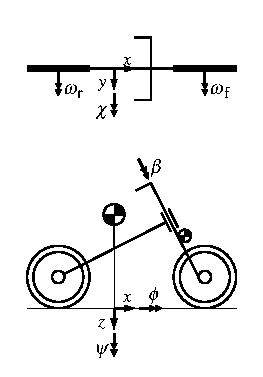
\includegraphics[width=55mm]{figure1}
  \caption{An example of a figure caption. Use 10~pt Times New Roman.
           For long captions, use a text width of 13~cm.
           Use the same style for the tables.} \label{fig:fig1}
\end{center}
\end{figure}
Figures, graphs and tables must be included in the same style as shown for 
Figure~\ref{fig:fig1} and Table~\ref{tab:tab1}.


\subsection{References}

Bibliographical citations should be written in the order in which they are 
cited, see the References section below, where Reference~\cite{Pac02} 
exemplifies the case of a textbook, while Reference~\cite{Ber07} is an article 
in conference proceedings and Reference~\cite{Sha71} is an article in a 
journal. Use can be made of a pre-existing bibtex style which uses a similar 
style.


\section{SUBMISSION OF PAPER}

The paper should be submitted by e-mail to \href{mailto:jbrendelson@bmd2016mke.org}{jbrendelson@bmd2016mke.org} with the email subject containing the phrase \textit{``BMD 2016 paper submission - submitting author last name''}. \uline{The deadline is September 1st, 2016}. The file of the paper must be in the Portable Document Format (PDF) and the file size should be within the limit of 10 MB. Exceptionally, other file formats can be accepted if the symposium organizers have been informed beforehand. 

Please make sure that the final version of the paper complies with the standards set here. Please note slightly different formatting requirements of the abstract and the final paper.

\section{CONCLUSIONS}

We very much look forward to welcoming you in Milwaukee! Best wishes and the 
warmest regards from the Organizing Committee of Bicycle and Motorcycle 
Dynamics 2016.

% \bibliographystyle{acm}
% \bibliography{biblio}
\begin{thebibliography}{6}
% \begin{thebibliography}{66} % use this for more than 9 references
\bibitem{Pac02} H.~B.~Pacejka,
\textit{Tyre and Vehicle Dynamics},
Butterworth and Heinemann, Oxford, 2002.

\bibitem{Ber07} E.~Bertolazzi, F.~Biral, M.~Da~Lio and V.~Cossalter,
``The influence of rider's upper body motions on motorcycle minimum time
  maneuvering'',
in C.~L.~Bottasso, P.~Masarati and L.~Trainelli (eds),
\textit{Proceedings, Multibody Dynamics 2007, ECCOMAS Thematic Conference},
Milano, Italy, 25--28 June 2007,
Politecnico di Milano, Milano, 2007, 15~pp.

\bibitem{Sha71} R.~S.~Sharp,
``The stability and control of motorcycles'',
\textit{Proceedings of the IMechE, Part C, Journal of Mechanical Engineering
  Science} \textbf{13} (1971), pp.~316--329.


\end{thebibliography}


\end{document}

